%%%%%%%%%%%%%%%%%%%%%%%%%%%%%%%%%%%%%%%%%
% University Assignment Title Page 
% LaTeX Template
% Version 1.0 (27/12/12)
%
% This template has been downloaded from:
% http://www.LaTeXTemplates.com
%
% Original author:
% WikiBooks (http://en.wikibooks.org/wiki/LaTeX/Title_Creation)
%
% License:
% CC BY-NC-SA 3.0 (http://creativecommons.org/licenses/by-nc-sa/3.0/)
% 
% Instructions for using this template:
% This title page is capable of being compiled as is. This is not useful for 
% including it in another document. To do this, you have two options: 
%
% 1) Copy/paste everything between \begin{document} and \end{document} 
% starting at \begin{titlepage} and paste this into another LaTeX file where you 
% want your title page.
% OR
% 2) Remove everything outside the \begin{titlepage} and \end{titlepage} and 
% move this file to the same directory as the LaTeX file you wish to add it to. 
% Then add %%%%%%%%%%%%%%%%%%%%%%%%%%%%%%%%%%%%%%%%%
% University Assignment Title Page 
% LaTeX Template
% Version 1.0 (27/12/12)
%
% This template has been downloaded from:
% http://www.LaTeXTemplates.com
%
% Original author:
% WikiBooks (http://en.wikibooks.org/wiki/LaTeX/Title_Creation)
%
% License:
% CC BY-NC-SA 3.0 (http://creativecommons.org/licenses/by-nc-sa/3.0/)
% 
% Instructions for using this template:
% This title page is capable of being compiled as is. This is not useful for 
% including it in another document. To do this, you have two options: 
%
% 1) Copy/paste everything between \begin{document} and \end{document} 
% starting at \begin{titlepage} and paste this into another LaTeX file where you 
% want your title page.
% OR
% 2) Remove everything outside the \begin{titlepage} and \end{titlepage} and 
% move this file to the same directory as the LaTeX file you wish to add it to. 
% Then add %%%%%%%%%%%%%%%%%%%%%%%%%%%%%%%%%%%%%%%%%
% University Assignment Title Page 
% LaTeX Template
% Version 1.0 (27/12/12)
%
% This template has been downloaded from:
% http://www.LaTeXTemplates.com
%
% Original author:
% WikiBooks (http://en.wikibooks.org/wiki/LaTeX/Title_Creation)
%
% License:
% CC BY-NC-SA 3.0 (http://creativecommons.org/licenses/by-nc-sa/3.0/)
% 
% Instructions for using this template:
% This title page is capable of being compiled as is. This is not useful for 
% including it in another document. To do this, you have two options: 
%
% 1) Copy/paste everything between \begin{document} and \end{document} 
% starting at \begin{titlepage} and paste this into another LaTeX file where you 
% want your title page.
% OR
% 2) Remove everything outside the \begin{titlepage} and \end{titlepage} and 
% move this file to the same directory as the LaTeX file you wish to add it to. 
% Then add %%%%%%%%%%%%%%%%%%%%%%%%%%%%%%%%%%%%%%%%%
% University Assignment Title Page 
% LaTeX Template
% Version 1.0 (27/12/12)
%
% This template has been downloaded from:
% http://www.LaTeXTemplates.com
%
% Original author:
% WikiBooks (http://en.wikibooks.org/wiki/LaTeX/Title_Creation)
%
% License:
% CC BY-NC-SA 3.0 (http://creativecommons.org/licenses/by-nc-sa/3.0/)
% 
% Instructions for using this template:
% This title page is capable of being compiled as is. This is not useful for 
% including it in another document. To do this, you have two options: 
%
% 1) Copy/paste everything between \begin{document} and \end{document} 
% starting at \begin{titlepage} and paste this into another LaTeX file where you 
% want your title page.
% OR
% 2) Remove everything outside the \begin{titlepage} and \end{titlepage} and 
% move this file to the same directory as the LaTeX file you wish to add it to. 
% Then add \input{./title_page_1.tex} to your LaTeX file where you want your
% title page.
%
%%%%%%%%%%%%%%%%%%%%%%%%%%%%%%%%%%%%%%%%%

%----------------------------------------------------------------------------------------
%	PACKAGES AND OTHER DOCUMENT CONFIGURATIONS
%----------------------------------------------------------------------------------------

\documentclass[12pt]{report}
\usepackage{graphicx}
\usepackage[section]{placeins}
\begin{document}

\begin{titlepage}

\newcommand{\HRule}{\rule{\linewidth}{0.5mm}} % Defines a new command for the horizontal lines, change thickness here

\center % Center everything on the page
 
%----------------------------------------------------------------------------------------
%	HEADING SECTIONS
%----------------------------------------------------------------------------------------
\textsc{\large Project Report On }\\[0.5cm] % Major heading such as course name % Minor heading such as course title

%----------------------------------------------------------------------------------------
%	TITLE SECTION
%----------------------------------------------------------------------------------------


{\Large  \bfseries EYE GAZE TRACKING
}\\[0.8cm] % Title of your document

\small \emph{Submitted in partial fulfillment of\\
        the requirements for the award of the degree of}
        \vspace{.2in}

       {\bf Bachelor of Technology \\in\\ Computer Science and Engineering}\\[0.2in]

 
%----------------------------------------------------------------------------------------
%	AUTHOR SECTION
%----------------------------------------------------------------------------------------
\textit{By}

\HRule \\[.2cm]
\begin{minipage}{0.4\textwidth}
\begin{flushleft} \large
Aravind Balakrishnan\\
Arun Abraham\\
Nikhil M S
\end{flushleft}
\end{minipage}
~
\begin{minipage}{0.4\textwidth}
\begin{flushright} \large
B100290CS\\
B100439CS\\
B100479CS\\
\end{flushright}
\end{minipage}\\[.5cm]

\HRule \\[0.2cm]

%----------------------------------------------------------------------------------------
%	Guidance
%----------------------------------------------------------------------------------------
\textit{\textit{Under the guidance of}}\\[0.1cm]
\textbf{\large Mrs. Lijiya A}\\[0.4cm]
%----------------------------------------------------------------------------------------
%	Image logo
%----------------------------------------------------------------------------------------

\includegraphics[scale=0.25]{nitc}\\
\Large { \textit \textbf Computer Science And Engineering}\\
 \large {NATIONAL INSTITUTE OF TECHNOLOGY CALICUT}
 Calicut, Kerala 673601
%----------------------------------------------------------------------------------------
%	DATE SECTION
%----------------------------------------------------------------------------------------

\textit{\large Winter Semester 2014}\\[3cm] % Date, change the \today to a set date if you want to be precise

%----------------------------------------------------------------------------------------
%	LOGO SECTION
%----------------------------------------------------------------------------------------

%\includegraphics{Logo}\\[1cm] % Include a department/university logo - this will require the graphicx package
 
%----------------------------------------------------------------------------------------

\vfill % Fill the rest of the page with whitespace

\end{titlepage}
%------------------------------------Certificate---------------------------------------------------

\newpage
\thispagestyle{empty}

\begin{center}

\huge{Computer Science and Engineering}\\
\normalsize
\textsc{National Institute of Technology Calicut}\\[2cm]

\emph{\LARGE Certificate}\\[2.0cm]
\end{center}
\normalsize This is to certify that the project work entitled "Eye Gaze Tracking", submitted by the following students to National Institute of Technology Calicut towards partial fulfilment of the requirements of the award of Degree Of Bachelor of Technology in Computer Science and Engineering is a bonafide record of the work carried out by them under my supervision and guidance.\\[.5cm]

\begin{table}[h]
\centering
\begin{tabular}{lr}
Roll No & Names of Students  \\ \hline
\\
B100290CS & Aravind Balakrishnan \\
B100439CS & Arun Abraham \\ 
B100479CS & Nikhil M S \\
\\
\hline
\end{tabular}
\end{table}

\vfill


% Bottom of the page
\begin{flushright}
Mrs. Lijiya A\\
(Project Guide)\\[1.5cm]
Gopakumar G\\
(Course Coordinator)\\
\end{flushright}

\begin{flushleft}
Place: Calicut \\
Date:

\end{flushleft}

%------------------------------------End of Certificate----------------------------------------------

\v
\begin{abstract}

 American film studios collectively produce several hundred movies every year, making the United States the third most prolific producer of films in the world. The budget of these movies is of the order of hundreds of millions of dollars, making their box office success absolutely essential for the survival of the industry. Knowing which movies are likely to succeed and which are likely to fail before the release could benefit the production houses greatly as it will enable them to focus their advertising campaigns which itself cost millions of dollars, accordingly. And it could also help them to know when it is most appropriate to release a movie by looking at the overall market. So the prediction of movie success is of great importance to the industry.

Machine learning algorithms are widely used to make predictions such as growth in the stock market, demand for products, nature of tumors etc. The goal of this project is to use data available in the Internet to predict the revenue of the movies and the critical success as well. Critical success will be represented by the IMDB ratings. The main challenge is to find the appropriate features to be considered for making the predictions. This problem is modelled as a linear regression problem.

\end{abstract}
\clearpage
\chapter*{PROBLEM STATEMENT}
The aim of the project is to predict the box office revenue and critical success of new Hollywood movies using machine learning techniques. The IMDB rating after at least one month after the release is considered as the index of critical success. We intend to make two predictions, one before the release and the second after one week of release. 
\clearpage
\pagenumbering{roman}
\tableofcontents
\newpage
\pagenumbering{arabic}
\chapter{INTRODUCTION}
In the United States of America 1000s of films are released every year.Since the 1920s, the American film industry has grossed more money every year than that of any other country. Cinema in America is a multi-billion dollar industry where even individual films earn over a billion dollars. Large production houses control most of the film industry, with billions of dollars spent on advertisements alone. Advertising campaigns contribute heavily to the total budget of the movies. Sometimes the investment results in heavy losses to the producers.
Warner Brothers, one of the largest production houses had a fall in their revenues last year despite the inflation and the increased number of movies released. If it was somehow possible to know beforehand the likelihood of success of the movies, the production houses could adjust the release of their movies so as to gain maximum profit. They could use the predictions to know when the market is dull and when its not.
 This shows a dire need for such a software to be developed. Many have tried to accomplish this goal of predicting movie revenues. Techniques such as social media sentiment analysis have been used in the past. None of the studies thus far has succeeded in suggesting a model good enough to be used in the industry.
In this project we attempt to use IMDB data to predict the gross revenue of the movies as well as their IMDB rating.


\clearpage
\chapter{LITERATURE SURVEY}
Lot of work has been done in the area and too many people have attempted to use statistics in combination with machine learning algorithms to predict various entities.\\
\begin{itemize}
\item Opinion Finder, a project conducted at University of Pittsburg [5] attempted to  use tweets to predict market sentiments. Their approach was to give different weightage to the adjectives in the tweets. They assigned values ranging from +2 to -2 to certain words and took the average weight to make predictions.
\item In their paper presented in the 49th annual meeting for ACN in 2011 [6]. Andrew Ng, Christopher Potts and their colleagues pointed out the importance of using a mix of supervised and unsupervised  approaches to learn word vectors capturing semantic term–document information as well as rich sentiment content.
\item Independant works conducted by Matts Forsell and Darin Im [3] attempted to predict Movie Revenues and had different success rates. Forsell’s prediction used a slightly more extensive training set than Im’s. But the prediction success was lower. Darin Im used a smaller training set, however used data that was from very recent movies. Forsell noted that error rates were significantly higher in predicting success of movies with budget lower than 100 million. 
\item Project conducted by Deniz Demir and Olga Kapralova at Stanford [7] used google trends statistics to improve movie gross prediction. They tried two different approaches. In one they used google trends statistics in combination with google adwords, in the other they used google trends statistics only.Their data set consisted of 800 movies only. This was mainly because google trends statistics  is available from 2004 onwards only. They used Logistic Regression, SVM and Multilayer perceptron approaches. All three approaches yielded average success rate close to 50 percentage. However, SVM method correctly predicted 98\% of the low rated movies but its success rate for high rated movies(ratings above 6) was a meagre 11\%.

\item Wenbin Zhang at Sony Brook University,NY used news analysis [8] alone to predict movie revenues without considering any other parameters including IMDB data. In their approach they tried to find correlations between various parameters and movie revenues. They found that prediction models using news data only can achieve similar performance to models using IMDB data, especially for high-grossing movies. They concluded that adding news analysis features can improve performance of predictions that use IMDB data alone.
\end{itemize}
\clearpage

\chapter{DESIGN}
\begin{figure}[h!]
  \centering
      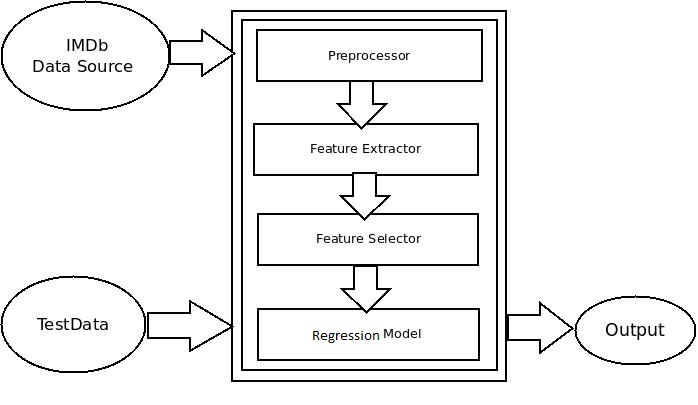
\includegraphics[scale=0.7]{Diagram.jpg}
  \caption{General Design}
\end{figure}
\section{Introduction}
The project can be mainly divided into two stages
\begin{description}
\item[$\bullet$ ]Dataset Collection and Preprocessing.
\item[$\bullet$ ]Construction of Regression Model.
\end{description}
\section{Dataset Collection and Preprocessing}
Dataset Collection is an important step in all machine learning problems. Preprocessing includes feature extraction and selection.
\subsection{Dataset Collection}
The initial dataset to be used will be collected from IMDb. It will consist of movies that were released from 2000 to 2012. Among these movies,we only selected the ones that were released in the United States and are in English, in the anticipation that we would be able to make more accurate predictions on these movies given that their reviews would also be in English.We removed movies which don't have any information about Box office details. 
\subsection{Preprocessing}


In preprocessing step we intent to eliminate training samples that have insufficient data. Also we intent to ensure that all the 19 genres in the IMDB database are well represented. We also want to filter the data in order to remove redundant and unnecessary information.
\subsection{Feature Selection}
\begin{figure}[htb!]
  \centering
      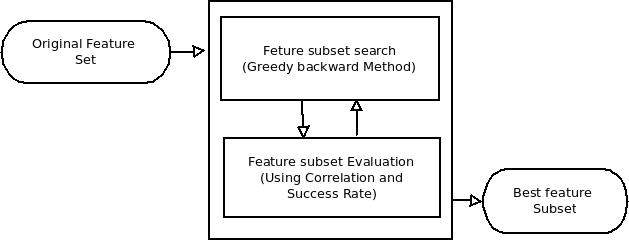
\includegraphics[scale=0.55]{featureselection.jpeg}
  \caption{Feature Selection}
\end{figure}
Here we look for correlation between all the different features under consideration and look for correlations with the target variable, ie movie revenue in dollars. We also look for correlation between the features themselves in order to avoid redundancy and irrelevant attributes. Also the extent of correlation is noted.Here we are using {\bf greedy 
backward procedure} to get best feature subset. The procedure starts with the
 full set of attributes.At each step, it removes the worst attribute remaining in the set.
At the end of the process, features that are not correlated to the target variable and those which are redundant are eliminated.

\section{Construction of Regression Model}
Supervised learning technique is adopted for this project.
We are using three models to predict the revenue and we will compare the performance of the different methods.




\subsection{Linear Regression Model}
In our first model, we use standard least-squares linear regression. To do this, we intend to use stochastic gradient descent. Once we have trained a set of feature weights, we could then generate gross revenue predictions as follows:
\centerline{ Gross = $\theta_{0}$ + $\theta_{1}$ * F$_1$ + $\theta_{2}$ * F$_2$ + ... + $\theta_{n}$ * F$_n$}\\	
where $\theta_i$ are the weights, F$_i$ are the features, and n is the number of features.\\
\subsection{Logistic Regression model}
We chose Logistic regression as our second method mainly because it generates a multi-class model with linear weights, most directly comparable to the feature weights given by linear regression. To define our classes we draw a histogram of movie revenues to create different buckets for prediction. These buckets are continuous ranges of movie revenues which covers the entire sample space.
\subsection{Support Vector Machine Regression Model}
SVMs can also be applied to regression problems.
SVM Regression try to find a function f(x)that has at most $\varepsilon$  deviation from the actually obtained targets y for all the training data, and at the same time is as flat as possibles. SVM Regression do not care about errors as long as they are less than $\varepsilon$ .We used linear kernel function to  map the data into a high dimensional feature space where linear regression is performed.
\clearpage
\chapter{WORK DONE}

\section{Obtaining The Data Set}
\begin{figure}[htb!]
  \centering
      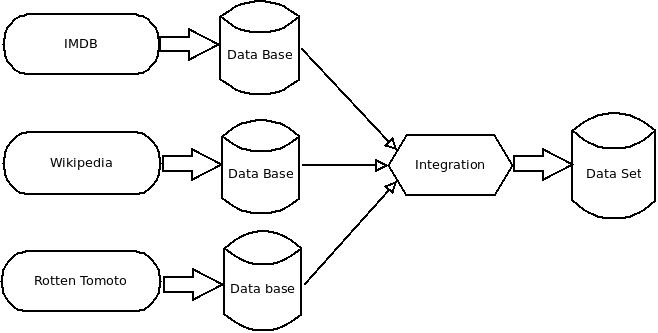
\includegraphics[scale=0.55]{data.jpeg}
  \caption{Data Collection and Integration}
\end{figure}
The data for a subset of movies,actors,reviews is provided by imdb via an alternative interface. Python scripts could be used to obtain data from IMDB. The data regarding each movie is spread over two web pages. The main page(imdb.com/title/movieid.html) and box office page.  
The data is also available at other websites like OMDB and Rotten Tomatoes in JSON format.
Eventually we faced a problem with Budget information.
Budget data is not provided by both IMDB and  Rotten Tomatoes. So we used wikipedia to obtain Budget details.
\section {Data Preprocessing}
The data we obtained are highly suseptible to noisy, missing and inconsistent data due to huge size and their likely origin from multiple, heterogeneous sources[9]. We mainly used IMDB and Rotten Tomatoes and Wikipedia. The main problem  with datasets were missing fields. To overcome this missing field problem we adopted a method which uses a measure of central tendency for the attribute. We used both mean and median as central tendency. Then removed duplicate entries.
\subsection {Data Integration}
Data obtained from three different resources IMDB, Wikipedia and Rotten Tomatoes was then  integrated into one database.
\subsection {Data Transformation}
In this step integrated data are transformed or consolidated so that the regression process may be more efficient and easier.
Dataset is mixed with both nominal and numeric attributes but for regression process we need all attributes to be numerical.
We used a measure of central tendency of Box office revenue to convert corresponding nominal attributes to numerical.
\subsection{Selecting feature Subset}
The dataset contained 20 features. We implemented a greedy backward procedure to reduce the dataset to the best feature subset. This resulted in a subset of 7 features.
\subsection{Measuring Sentiment Score From Reviews}
WE implemented a module to compute sentiment scores using a technique similar to the one used in the opinion finder project. The method involves assigning weights to commonly used adjectives to obtain an average weight.
\clearpage
\section{MACHINE LEARNING}
\subsection {Building a Linear Regression Model}
Using the method of Normal equation we built a linear regression model. We used data regarding 950 films  for training purpose and 100 for testing.Initially we had 17 features in the data set. After feature selection we chose a training set with the seven features that showed highest correlation to the target variable and low correlation among themselves. Correlation between features and cross validation on the training data were used as the performance matrix.


\subsection {Logistic Regression model}
   For logistic regression to apply we need to change the problem which is a regression problem to a classification problem. To achieve this we split the range of the target variable into a finite number of buckets of equal size. We found that the target variable takes values between \$2100 and \$436500000. We also found that only a few movies grossed over \$100 million. So we decided not to consider the movies that grossed over  \$100 million in the training set for the logistic regression model. We modelled the problem as a four class classification problem. The four classes were from \$0-\$25, \$25-\$50, \$50-\$75, \$75-\$100. There were a total of 876 movies in the data-set and we used 776 for training and 100 for testing. We used gradient descent algorithm to find the weights of the features.
\subsection {SVM with Linear Kernel}
Since Training data is not large as compared to number of features, we used linear kernel function. $\varepsilon$ was set to 0.1 and Hyperparameter C optimization was done using grid search.Grid search is exhaustive search through a manually specified subset of the hyperparameter space.Cross validation on the training was used as the performance matrix .The Optimum value for C was found to be 0.1 .
\\
\\

\section{WEB APPLICATION}
A web application was built using python to make results available to public.
\subsection {Google App engine}
Google App engine is used as the platform to run the code and is shared among the public to utilize the application.
\subsection {OMBD API}
Omdb API is used to collect the preliminary data set. Using this API we collected English movies from 2000 to 2010. We got around 25000 movies in the json format.
\subsection {Wikipedia}
Data set we collected using Omdb Api did not have the information regarding the budget of the films.To collect this information we used Wikipedia to collect budget data about films.
\clearpage


\chapter{RESULT}
The result we found out using Linear regression was about 51\% accurate. Where As for logistic regression we got 42.2\% accuracy which is a comparatively low result. SVM approach had a success rate of 39\%. The error tolerance for SVM and Linear regression was 20\%. For logistic regression the error tolerance was 12.5\%. Of all the 20 features in the data-set, budget, director, writer, actor1, actor2, gender, tomato reviews were found to be the most significant features.

\begin{center}
    \begin{tabular}{ | l | l | l | p{5cm} |}
    \hline
    Model & Linear Regression & Logistic Regression & SVM \\ \hline
    Tolerance & 20\% & 12.5\% & 20\% \\ \hline
    Success Rate & 50.7\% & 42.2\% & 39.0\% \\ \hline
    Correlation & 0.965 & - & 0.956 \\ \hline
    \end{tabular}
\end{center}



\chapter{CONCLUSION}
After building the three models we found out that the linear model represents the movie features most accurately. The success percentage for all models, while not good enough for industrial use, are in the close proximity of values obtained in previous studies. Some of the results obtained are better than that of some standard libraries and similar studies. Even though not good enough for industrial purposes the models built can be used in online applications.


A regression model which is supplied with a larger training set will be able to perform better. More data can be added to the training set over time as new information becomes available.

%% ADD data
\chapter{FUTURE WORKS}
\begin{description}
A larger training set is the key to improving the performance of the model. We need to consider additional features to achieve this. News analysis and plot analysis could be done and the information thus obtained could be added to the training set.

\end{description}

%\clearpage
\begin{thebibliography}{10}
\addcontentsline{toc}{chapter}{BIBLIOGRAPHY}
\bibitem{latexGuide} Richard O. Duda, Peter E. Hart, David G.
Stork,{\it Pattern Classification}, 2nd ed.NewYork: Wiley, 1973


\bibitem{latexMath}Sagar V. Mehta, Rose Marie Philip, Aju Thalappillil Scaria, "Predicting Movie Rating based on Text Reviews," Dept.Elect.Eng, Stanford Univ., California, December, 2011


\bibitem{latexGuide}Darin Im, Minh Thao, Dang Nguyen, "Predicting Movie Success in the U.S. market," Dept.Elect.Eng, Stanford Univ., California, December, 2011
 



\bibitem{latexMath}Suhaas Prasad, "Using Social Networks to improve Movie Ratings predictions,"
Dept.Elect.Eng, Stanford Univ., California, 2010

\bibitem{latexMath}Opinion Finder Project, University of Pittsburg,
Available: http://mpqa.cs.pitt.edu/opinionfinder/


\bibitem{latexMath}Andrew L. Maas, Raymond E. Daly, Peter T. Pham, Dan Huang,
Andrew Y. Ng, and Christopher Potts, "Learning Word Vectors for Sentiment Analysis,"In Proc. 49th Annual Meeting of the Association for Computational Linguistics, Oregon, 2011, pp 142$-$150


\bibitem{latexMath} Deniz Demir, Olga Kapralova, Hongze Lai, "Predicting IMDB Movie Ratings Using Google Trends," Dept.Elect.Eng, Stanford Univ., California, December, 2012

\bibitem{latexMath}W. Zhang and S. Skiena," Improving movie gross prediction through news analysis,", IEEE/WIC/ACM International Conference on Web Intelligence and Intelligent Agent Technology, Milan, 2009\\

\bibitem{latexMath} Jiawei Han, Micheline Kamber, Jian Pei,{\it  Data Mining Concepts and Techniques}, 3rd ed.MA:Elsevier, 2011, pp. 83-117
\end{thebibliography}
\end{document} to your LaTeX file where you want your
% title page.
%
%%%%%%%%%%%%%%%%%%%%%%%%%%%%%%%%%%%%%%%%%

%----------------------------------------------------------------------------------------
%	PACKAGES AND OTHER DOCUMENT CONFIGURATIONS
%----------------------------------------------------------------------------------------

\documentclass[12pt]{report}
\usepackage{graphicx}
\usepackage[section]{placeins}
\begin{document}

\begin{titlepage}

\newcommand{\HRule}{\rule{\linewidth}{0.5mm}} % Defines a new command for the horizontal lines, change thickness here

\center % Center everything on the page
 
%----------------------------------------------------------------------------------------
%	HEADING SECTIONS
%----------------------------------------------------------------------------------------
\textsc{\large Project Report On }\\[0.5cm] % Major heading such as course name % Minor heading such as course title

%----------------------------------------------------------------------------------------
%	TITLE SECTION
%----------------------------------------------------------------------------------------


{\Large  \bfseries EYE GAZE TRACKING
}\\[0.8cm] % Title of your document

\small \emph{Submitted in partial fulfillment of\\
        the requirements for the award of the degree of}
        \vspace{.2in}

       {\bf Bachelor of Technology \\in\\ Computer Science and Engineering}\\[0.2in]

 
%----------------------------------------------------------------------------------------
%	AUTHOR SECTION
%----------------------------------------------------------------------------------------
\textit{By}

\HRule \\[.2cm]
\begin{minipage}{0.4\textwidth}
\begin{flushleft} \large
Aravind Balakrishnan\\
Arun Abraham\\
Nikhil M S
\end{flushleft}
\end{minipage}
~
\begin{minipage}{0.4\textwidth}
\begin{flushright} \large
B100290CS\\
B100439CS\\
B100479CS\\
\end{flushright}
\end{minipage}\\[.5cm]

\HRule \\[0.2cm]

%----------------------------------------------------------------------------------------
%	Guidance
%----------------------------------------------------------------------------------------
\textit{\textit{Under the guidance of}}\\[0.1cm]
\textbf{\large Mrs. Lijiya A}\\[0.4cm]
%----------------------------------------------------------------------------------------
%	Image logo
%----------------------------------------------------------------------------------------

\includegraphics[scale=0.25]{nitc}\\
\Large { \textit \textbf Computer Science And Engineering}\\
 \large {NATIONAL INSTITUTE OF TECHNOLOGY CALICUT}
 Calicut, Kerala 673601
%----------------------------------------------------------------------------------------
%	DATE SECTION
%----------------------------------------------------------------------------------------

\textit{\large Winter Semester 2014}\\[3cm] % Date, change the \today to a set date if you want to be precise

%----------------------------------------------------------------------------------------
%	LOGO SECTION
%----------------------------------------------------------------------------------------

%\includegraphics{Logo}\\[1cm] % Include a department/university logo - this will require the graphicx package
 
%----------------------------------------------------------------------------------------

\vfill % Fill the rest of the page with whitespace

\end{titlepage}
%------------------------------------Certificate---------------------------------------------------

\newpage
\thispagestyle{empty}

\begin{center}

\huge{Computer Science and Engineering}\\
\normalsize
\textsc{National Institute of Technology Calicut}\\[2cm]

\emph{\LARGE Certificate}\\[2.0cm]
\end{center}
\normalsize This is to certify that the project work entitled "Eye Gaze Tracking", submitted by the following students to National Institute of Technology Calicut towards partial fulfilment of the requirements of the award of Degree Of Bachelor of Technology in Computer Science and Engineering is a bonafide record of the work carried out by them under my supervision and guidance.\\[.5cm]

\begin{table}[h]
\centering
\begin{tabular}{lr}
Roll No & Names of Students  \\ \hline
\\
B100290CS & Aravind Balakrishnan \\
B100439CS & Arun Abraham \\ 
B100479CS & Nikhil M S \\
\\
\hline
\end{tabular}
\end{table}

\vfill


% Bottom of the page
\begin{flushright}
Mrs. Lijiya A\\
(Project Guide)\\[1.5cm]
Gopakumar G\\
(Course Coordinator)\\
\end{flushright}

\begin{flushleft}
Place: Calicut \\
Date:

\end{flushleft}

%------------------------------------End of Certificate----------------------------------------------

\v
\begin{abstract}

 American film studios collectively produce several hundred movies every year, making the United States the third most prolific producer of films in the world. The budget of these movies is of the order of hundreds of millions of dollars, making their box office success absolutely essential for the survival of the industry. Knowing which movies are likely to succeed and which are likely to fail before the release could benefit the production houses greatly as it will enable them to focus their advertising campaigns which itself cost millions of dollars, accordingly. And it could also help them to know when it is most appropriate to release a movie by looking at the overall market. So the prediction of movie success is of great importance to the industry.

Machine learning algorithms are widely used to make predictions such as growth in the stock market, demand for products, nature of tumors etc. The goal of this project is to use data available in the Internet to predict the revenue of the movies and the critical success as well. Critical success will be represented by the IMDB ratings. The main challenge is to find the appropriate features to be considered for making the predictions. This problem is modelled as a linear regression problem.

\end{abstract}
\clearpage
\chapter*{PROBLEM STATEMENT}
The aim of the project is to predict the box office revenue and critical success of new Hollywood movies using machine learning techniques. The IMDB rating after at least one month after the release is considered as the index of critical success. We intend to make two predictions, one before the release and the second after one week of release. 
\clearpage
\pagenumbering{roman}
\tableofcontents
\newpage
\pagenumbering{arabic}
\chapter{INTRODUCTION}
In the United States of America 1000s of films are released every year.Since the 1920s, the American film industry has grossed more money every year than that of any other country. Cinema in America is a multi-billion dollar industry where even individual films earn over a billion dollars. Large production houses control most of the film industry, with billions of dollars spent on advertisements alone. Advertising campaigns contribute heavily to the total budget of the movies. Sometimes the investment results in heavy losses to the producers.
Warner Brothers, one of the largest production houses had a fall in their revenues last year despite the inflation and the increased number of movies released. If it was somehow possible to know beforehand the likelihood of success of the movies, the production houses could adjust the release of their movies so as to gain maximum profit. They could use the predictions to know when the market is dull and when its not.
 This shows a dire need for such a software to be developed. Many have tried to accomplish this goal of predicting movie revenues. Techniques such as social media sentiment analysis have been used in the past. None of the studies thus far has succeeded in suggesting a model good enough to be used in the industry.
In this project we attempt to use IMDB data to predict the gross revenue of the movies as well as their IMDB rating.


\clearpage
\chapter{LITERATURE SURVEY}
Lot of work has been done in the area and too many people have attempted to use statistics in combination with machine learning algorithms to predict various entities.\\
\begin{itemize}
\item Opinion Finder, a project conducted at University of Pittsburg [5] attempted to  use tweets to predict market sentiments. Their approach was to give different weightage to the adjectives in the tweets. They assigned values ranging from +2 to -2 to certain words and took the average weight to make predictions.
\item In their paper presented in the 49th annual meeting for ACN in 2011 [6]. Andrew Ng, Christopher Potts and their colleagues pointed out the importance of using a mix of supervised and unsupervised  approaches to learn word vectors capturing semantic term–document information as well as rich sentiment content.
\item Independant works conducted by Matts Forsell and Darin Im [3] attempted to predict Movie Revenues and had different success rates. Forsell’s prediction used a slightly more extensive training set than Im’s. But the prediction success was lower. Darin Im used a smaller training set, however used data that was from very recent movies. Forsell noted that error rates were significantly higher in predicting success of movies with budget lower than 100 million. 
\item Project conducted by Deniz Demir and Olga Kapralova at Stanford [7] used google trends statistics to improve movie gross prediction. They tried two different approaches. In one they used google trends statistics in combination with google adwords, in the other they used google trends statistics only.Their data set consisted of 800 movies only. This was mainly because google trends statistics  is available from 2004 onwards only. They used Logistic Regression, SVM and Multilayer perceptron approaches. All three approaches yielded average success rate close to 50 percentage. However, SVM method correctly predicted 98\% of the low rated movies but its success rate for high rated movies(ratings above 6) was a meagre 11\%.

\item Wenbin Zhang at Sony Brook University,NY used news analysis [8] alone to predict movie revenues without considering any other parameters including IMDB data. In their approach they tried to find correlations between various parameters and movie revenues. They found that prediction models using news data only can achieve similar performance to models using IMDB data, especially for high-grossing movies. They concluded that adding news analysis features can improve performance of predictions that use IMDB data alone.
\end{itemize}
\clearpage

\chapter{DESIGN}
\begin{figure}[h!]
  \centering
      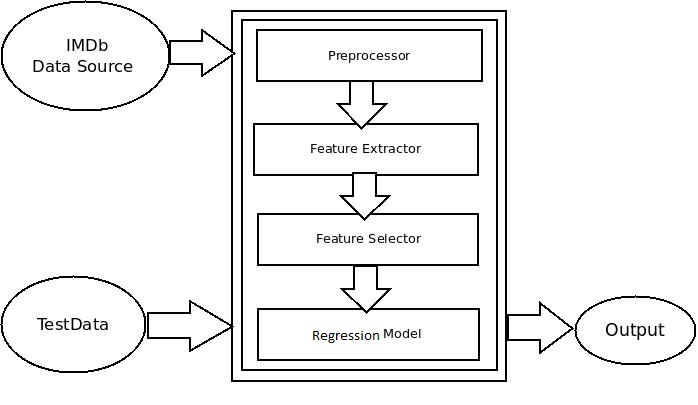
\includegraphics[scale=0.7]{Diagram.jpg}
  \caption{General Design}
\end{figure}
\section{Introduction}
The project can be mainly divided into two stages
\begin{description}
\item[$\bullet$ ]Dataset Collection and Preprocessing.
\item[$\bullet$ ]Construction of Regression Model.
\end{description}
\section{Dataset Collection and Preprocessing}
Dataset Collection is an important step in all machine learning problems. Preprocessing includes feature extraction and selection.
\subsection{Dataset Collection}
The initial dataset to be used will be collected from IMDb. It will consist of movies that were released from 2000 to 2012. Among these movies,we only selected the ones that were released in the United States and are in English, in the anticipation that we would be able to make more accurate predictions on these movies given that their reviews would also be in English.We removed movies which don't have any information about Box office details. 
\subsection{Preprocessing}


In preprocessing step we intent to eliminate training samples that have insufficient data. Also we intent to ensure that all the 19 genres in the IMDB database are well represented. We also want to filter the data in order to remove redundant and unnecessary information.
\subsection{Feature Selection}
\begin{figure}[htb!]
  \centering
      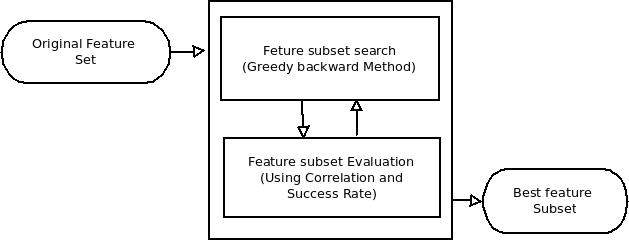
\includegraphics[scale=0.55]{featureselection.jpeg}
  \caption{Feature Selection}
\end{figure}
Here we look for correlation between all the different features under consideration and look for correlations with the target variable, ie movie revenue in dollars. We also look for correlation between the features themselves in order to avoid redundancy and irrelevant attributes. Also the extent of correlation is noted.Here we are using {\bf greedy 
backward procedure} to get best feature subset. The procedure starts with the
 full set of attributes.At each step, it removes the worst attribute remaining in the set.
At the end of the process, features that are not correlated to the target variable and those which are redundant are eliminated.

\section{Construction of Regression Model}
Supervised learning technique is adopted for this project.
We are using three models to predict the revenue and we will compare the performance of the different methods.




\subsection{Linear Regression Model}
In our first model, we use standard least-squares linear regression. To do this, we intend to use stochastic gradient descent. Once we have trained a set of feature weights, we could then generate gross revenue predictions as follows:
\centerline{ Gross = $\theta_{0}$ + $\theta_{1}$ * F$_1$ + $\theta_{2}$ * F$_2$ + ... + $\theta_{n}$ * F$_n$}\\	
where $\theta_i$ are the weights, F$_i$ are the features, and n is the number of features.\\
\subsection{Logistic Regression model}
We chose Logistic regression as our second method mainly because it generates a multi-class model with linear weights, most directly comparable to the feature weights given by linear regression. To define our classes we draw a histogram of movie revenues to create different buckets for prediction. These buckets are continuous ranges of movie revenues which covers the entire sample space.
\subsection{Support Vector Machine Regression Model}
SVMs can also be applied to regression problems.
SVM Regression try to find a function f(x)that has at most $\varepsilon$  deviation from the actually obtained targets y for all the training data, and at the same time is as flat as possibles. SVM Regression do not care about errors as long as they are less than $\varepsilon$ .We used linear kernel function to  map the data into a high dimensional feature space where linear regression is performed.
\clearpage
\chapter{WORK DONE}

\section{Obtaining The Data Set}
\begin{figure}[htb!]
  \centering
      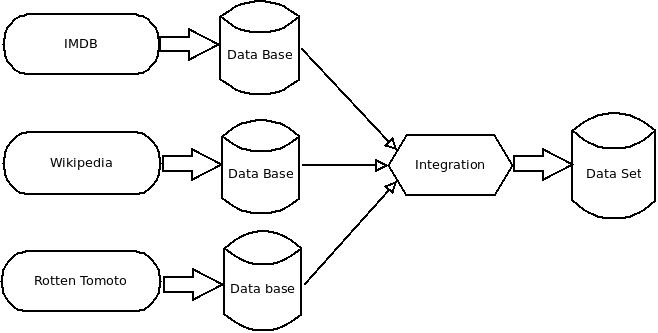
\includegraphics[scale=0.55]{data.jpeg}
  \caption{Data Collection and Integration}
\end{figure}
The data for a subset of movies,actors,reviews is provided by imdb via an alternative interface. Python scripts could be used to obtain data from IMDB. The data regarding each movie is spread over two web pages. The main page(imdb.com/title/movieid.html) and box office page.  
The data is also available at other websites like OMDB and Rotten Tomatoes in JSON format.
Eventually we faced a problem with Budget information.
Budget data is not provided by both IMDB and  Rotten Tomatoes. So we used wikipedia to obtain Budget details.
\section {Data Preprocessing}
The data we obtained are highly suseptible to noisy, missing and inconsistent data due to huge size and their likely origin from multiple, heterogeneous sources[9]. We mainly used IMDB and Rotten Tomatoes and Wikipedia. The main problem  with datasets were missing fields. To overcome this missing field problem we adopted a method which uses a measure of central tendency for the attribute. We used both mean and median as central tendency. Then removed duplicate entries.
\subsection {Data Integration}
Data obtained from three different resources IMDB, Wikipedia and Rotten Tomatoes was then  integrated into one database.
\subsection {Data Transformation}
In this step integrated data are transformed or consolidated so that the regression process may be more efficient and easier.
Dataset is mixed with both nominal and numeric attributes but for regression process we need all attributes to be numerical.
We used a measure of central tendency of Box office revenue to convert corresponding nominal attributes to numerical.
\subsection{Selecting feature Subset}
The dataset contained 20 features. We implemented a greedy backward procedure to reduce the dataset to the best feature subset. This resulted in a subset of 7 features.
\subsection{Measuring Sentiment Score From Reviews}
WE implemented a module to compute sentiment scores using a technique similar to the one used in the opinion finder project. The method involves assigning weights to commonly used adjectives to obtain an average weight.
\clearpage
\section{MACHINE LEARNING}
\subsection {Building a Linear Regression Model}
Using the method of Normal equation we built a linear regression model. We used data regarding 950 films  for training purpose and 100 for testing.Initially we had 17 features in the data set. After feature selection we chose a training set with the seven features that showed highest correlation to the target variable and low correlation among themselves. Correlation between features and cross validation on the training data were used as the performance matrix.


\subsection {Logistic Regression model}
   For logistic regression to apply we need to change the problem which is a regression problem to a classification problem. To achieve this we split the range of the target variable into a finite number of buckets of equal size. We found that the target variable takes values between \$2100 and \$436500000. We also found that only a few movies grossed over \$100 million. So we decided not to consider the movies that grossed over  \$100 million in the training set for the logistic regression model. We modelled the problem as a four class classification problem. The four classes were from \$0-\$25, \$25-\$50, \$50-\$75, \$75-\$100. There were a total of 876 movies in the data-set and we used 776 for training and 100 for testing. We used gradient descent algorithm to find the weights of the features.
\subsection {SVM with Linear Kernel}
Since Training data is not large as compared to number of features, we used linear kernel function. $\varepsilon$ was set to 0.1 and Hyperparameter C optimization was done using grid search.Grid search is exhaustive search through a manually specified subset of the hyperparameter space.Cross validation on the training was used as the performance matrix .The Optimum value for C was found to be 0.1 .
\\
\\

\section{WEB APPLICATION}
A web application was built using python to make results available to public.
\subsection {Google App engine}
Google App engine is used as the platform to run the code and is shared among the public to utilize the application.
\subsection {OMBD API}
Omdb API is used to collect the preliminary data set. Using this API we collected English movies from 2000 to 2010. We got around 25000 movies in the json format.
\subsection {Wikipedia}
Data set we collected using Omdb Api did not have the information regarding the budget of the films.To collect this information we used Wikipedia to collect budget data about films.
\clearpage


\chapter{RESULT}
The result we found out using Linear regression was about 51\% accurate. Where As for logistic regression we got 42.2\% accuracy which is a comparatively low result. SVM approach had a success rate of 39\%. The error tolerance for SVM and Linear regression was 20\%. For logistic regression the error tolerance was 12.5\%. Of all the 20 features in the data-set, budget, director, writer, actor1, actor2, gender, tomato reviews were found to be the most significant features.

\begin{center}
    \begin{tabular}{ | l | l | l | p{5cm} |}
    \hline
    Model & Linear Regression & Logistic Regression & SVM \\ \hline
    Tolerance & 20\% & 12.5\% & 20\% \\ \hline
    Success Rate & 50.7\% & 42.2\% & 39.0\% \\ \hline
    Correlation & 0.965 & - & 0.956 \\ \hline
    \end{tabular}
\end{center}



\chapter{CONCLUSION}
After building the three models we found out that the linear model represents the movie features most accurately. The success percentage for all models, while not good enough for industrial use, are in the close proximity of values obtained in previous studies. Some of the results obtained are better than that of some standard libraries and similar studies. Even though not good enough for industrial purposes the models built can be used in online applications.


A regression model which is supplied with a larger training set will be able to perform better. More data can be added to the training set over time as new information becomes available.

%% ADD data
\chapter{FUTURE WORKS}
\begin{description}
A larger training set is the key to improving the performance of the model. We need to consider additional features to achieve this. News analysis and plot analysis could be done and the information thus obtained could be added to the training set.

\end{description}

%\clearpage
\begin{thebibliography}{10}
\addcontentsline{toc}{chapter}{BIBLIOGRAPHY}
\bibitem{latexGuide} Richard O. Duda, Peter E. Hart, David G.
Stork,{\it Pattern Classification}, 2nd ed.NewYork: Wiley, 1973


\bibitem{latexMath}Sagar V. Mehta, Rose Marie Philip, Aju Thalappillil Scaria, "Predicting Movie Rating based on Text Reviews," Dept.Elect.Eng, Stanford Univ., California, December, 2011


\bibitem{latexGuide}Darin Im, Minh Thao, Dang Nguyen, "Predicting Movie Success in the U.S. market," Dept.Elect.Eng, Stanford Univ., California, December, 2011
 



\bibitem{latexMath}Suhaas Prasad, "Using Social Networks to improve Movie Ratings predictions,"
Dept.Elect.Eng, Stanford Univ., California, 2010

\bibitem{latexMath}Opinion Finder Project, University of Pittsburg,
Available: http://mpqa.cs.pitt.edu/opinionfinder/


\bibitem{latexMath}Andrew L. Maas, Raymond E. Daly, Peter T. Pham, Dan Huang,
Andrew Y. Ng, and Christopher Potts, "Learning Word Vectors for Sentiment Analysis,"In Proc. 49th Annual Meeting of the Association for Computational Linguistics, Oregon, 2011, pp 142$-$150


\bibitem{latexMath} Deniz Demir, Olga Kapralova, Hongze Lai, "Predicting IMDB Movie Ratings Using Google Trends," Dept.Elect.Eng, Stanford Univ., California, December, 2012

\bibitem{latexMath}W. Zhang and S. Skiena," Improving movie gross prediction through news analysis,", IEEE/WIC/ACM International Conference on Web Intelligence and Intelligent Agent Technology, Milan, 2009\\

\bibitem{latexMath} Jiawei Han, Micheline Kamber, Jian Pei,{\it  Data Mining Concepts and Techniques}, 3rd ed.MA:Elsevier, 2011, pp. 83-117
\end{thebibliography}
\end{document} to your LaTeX file where you want your
% title page.
%
%%%%%%%%%%%%%%%%%%%%%%%%%%%%%%%%%%%%%%%%%

%----------------------------------------------------------------------------------------
%	PACKAGES AND OTHER DOCUMENT CONFIGURATIONS
%----------------------------------------------------------------------------------------

\documentclass[12pt]{report}
\usepackage{graphicx}
\usepackage[section]{placeins}
\begin{document}

\begin{titlepage}

\newcommand{\HRule}{\rule{\linewidth}{0.5mm}} % Defines a new command for the horizontal lines, change thickness here

\center % Center everything on the page
 
%----------------------------------------------------------------------------------------
%	HEADING SECTIONS
%----------------------------------------------------------------------------------------
\textsc{\large Project Report On }\\[0.5cm] % Major heading such as course name % Minor heading such as course title

%----------------------------------------------------------------------------------------
%	TITLE SECTION
%----------------------------------------------------------------------------------------


{\Large  \bfseries EYE GAZE TRACKING
}\\[0.8cm] % Title of your document

\small \emph{Submitted in partial fulfillment of\\
        the requirements for the award of the degree of}
        \vspace{.2in}

       {\bf Bachelor of Technology \\in\\ Computer Science and Engineering}\\[0.2in]

 
%----------------------------------------------------------------------------------------
%	AUTHOR SECTION
%----------------------------------------------------------------------------------------
\textit{By}

\HRule \\[.2cm]
\begin{minipage}{0.4\textwidth}
\begin{flushleft} \large
Aravind Balakrishnan\\
Arun Abraham\\
Nikhil M S
\end{flushleft}
\end{minipage}
~
\begin{minipage}{0.4\textwidth}
\begin{flushright} \large
B100290CS\\
B100439CS\\
B100479CS\\
\end{flushright}
\end{minipage}\\[.5cm]

\HRule \\[0.2cm]

%----------------------------------------------------------------------------------------
%	Guidance
%----------------------------------------------------------------------------------------
\textit{\textit{Under the guidance of}}\\[0.1cm]
\textbf{\large Mrs. Lijiya A}\\[0.4cm]
%----------------------------------------------------------------------------------------
%	Image logo
%----------------------------------------------------------------------------------------

\includegraphics[scale=0.25]{nitc}\\
\Large { \textit \textbf Computer Science And Engineering}\\
 \large {NATIONAL INSTITUTE OF TECHNOLOGY CALICUT}
 Calicut, Kerala 673601
%----------------------------------------------------------------------------------------
%	DATE SECTION
%----------------------------------------------------------------------------------------

\textit{\large Winter Semester 2014}\\[3cm] % Date, change the \today to a set date if you want to be precise

%----------------------------------------------------------------------------------------
%	LOGO SECTION
%----------------------------------------------------------------------------------------

%\includegraphics{Logo}\\[1cm] % Include a department/university logo - this will require the graphicx package
 
%----------------------------------------------------------------------------------------

\vfill % Fill the rest of the page with whitespace

\end{titlepage}
%------------------------------------Certificate---------------------------------------------------

\newpage
\thispagestyle{empty}

\begin{center}

\huge{Computer Science and Engineering}\\
\normalsize
\textsc{National Institute of Technology Calicut}\\[2cm]

\emph{\LARGE Certificate}\\[2.0cm]
\end{center}
\normalsize This is to certify that the project work entitled "Eye Gaze Tracking", submitted by the following students to National Institute of Technology Calicut towards partial fulfilment of the requirements of the award of Degree Of Bachelor of Technology in Computer Science and Engineering is a bonafide record of the work carried out by them under my supervision and guidance.\\[.5cm]

\begin{table}[h]
\centering
\begin{tabular}{lr}
Roll No & Names of Students  \\ \hline
\\
B100290CS & Aravind Balakrishnan \\
B100439CS & Arun Abraham \\ 
B100479CS & Nikhil M S \\
\\
\hline
\end{tabular}
\end{table}

\vfill


% Bottom of the page
\begin{flushright}
Mrs. Lijiya A\\
(Project Guide)\\[1.5cm]
Gopakumar G\\
(Course Coordinator)\\
\end{flushright}

\begin{flushleft}
Place: Calicut \\
Date:

\end{flushleft}

%------------------------------------End of Certificate----------------------------------------------

\v
\begin{abstract}

 American film studios collectively produce several hundred movies every year, making the United States the third most prolific producer of films in the world. The budget of these movies is of the order of hundreds of millions of dollars, making their box office success absolutely essential for the survival of the industry. Knowing which movies are likely to succeed and which are likely to fail before the release could benefit the production houses greatly as it will enable them to focus their advertising campaigns which itself cost millions of dollars, accordingly. And it could also help them to know when it is most appropriate to release a movie by looking at the overall market. So the prediction of movie success is of great importance to the industry.

Machine learning algorithms are widely used to make predictions such as growth in the stock market, demand for products, nature of tumors etc. The goal of this project is to use data available in the Internet to predict the revenue of the movies and the critical success as well. Critical success will be represented by the IMDB ratings. The main challenge is to find the appropriate features to be considered for making the predictions. This problem is modelled as a linear regression problem.

\end{abstract}
\clearpage
\chapter*{PROBLEM STATEMENT}
The aim of the project is to predict the box office revenue and critical success of new Hollywood movies using machine learning techniques. The IMDB rating after at least one month after the release is considered as the index of critical success. We intend to make two predictions, one before the release and the second after one week of release. 
\clearpage
\pagenumbering{roman}
\tableofcontents
\newpage
\pagenumbering{arabic}
\chapter{INTRODUCTION}
In the United States of America 1000s of films are released every year.Since the 1920s, the American film industry has grossed more money every year than that of any other country. Cinema in America is a multi-billion dollar industry where even individual films earn over a billion dollars. Large production houses control most of the film industry, with billions of dollars spent on advertisements alone. Advertising campaigns contribute heavily to the total budget of the movies. Sometimes the investment results in heavy losses to the producers.
Warner Brothers, one of the largest production houses had a fall in their revenues last year despite the inflation and the increased number of movies released. If it was somehow possible to know beforehand the likelihood of success of the movies, the production houses could adjust the release of their movies so as to gain maximum profit. They could use the predictions to know when the market is dull and when its not.
 This shows a dire need for such a software to be developed. Many have tried to accomplish this goal of predicting movie revenues. Techniques such as social media sentiment analysis have been used in the past. None of the studies thus far has succeeded in suggesting a model good enough to be used in the industry.
In this project we attempt to use IMDB data to predict the gross revenue of the movies as well as their IMDB rating.


\clearpage
\chapter{LITERATURE SURVEY}
Lot of work has been done in the area and too many people have attempted to use statistics in combination with machine learning algorithms to predict various entities.\\
\begin{itemize}
\item Opinion Finder, a project conducted at University of Pittsburg [5] attempted to  use tweets to predict market sentiments. Their approach was to give different weightage to the adjectives in the tweets. They assigned values ranging from +2 to -2 to certain words and took the average weight to make predictions.
\item In their paper presented in the 49th annual meeting for ACN in 2011 [6]. Andrew Ng, Christopher Potts and their colleagues pointed out the importance of using a mix of supervised and unsupervised  approaches to learn word vectors capturing semantic term–document information as well as rich sentiment content.
\item Independant works conducted by Matts Forsell and Darin Im [3] attempted to predict Movie Revenues and had different success rates. Forsell’s prediction used a slightly more extensive training set than Im’s. But the prediction success was lower. Darin Im used a smaller training set, however used data that was from very recent movies. Forsell noted that error rates were significantly higher in predicting success of movies with budget lower than 100 million. 
\item Project conducted by Deniz Demir and Olga Kapralova at Stanford [7] used google trends statistics to improve movie gross prediction. They tried two different approaches. In one they used google trends statistics in combination with google adwords, in the other they used google trends statistics only.Their data set consisted of 800 movies only. This was mainly because google trends statistics  is available from 2004 onwards only. They used Logistic Regression, SVM and Multilayer perceptron approaches. All three approaches yielded average success rate close to 50 percentage. However, SVM method correctly predicted 98\% of the low rated movies but its success rate for high rated movies(ratings above 6) was a meagre 11\%.

\item Wenbin Zhang at Sony Brook University,NY used news analysis [8] alone to predict movie revenues without considering any other parameters including IMDB data. In their approach they tried to find correlations between various parameters and movie revenues. They found that prediction models using news data only can achieve similar performance to models using IMDB data, especially for high-grossing movies. They concluded that adding news analysis features can improve performance of predictions that use IMDB data alone.
\end{itemize}
\clearpage

\chapter{DESIGN}
\begin{figure}[h!]
  \centering
      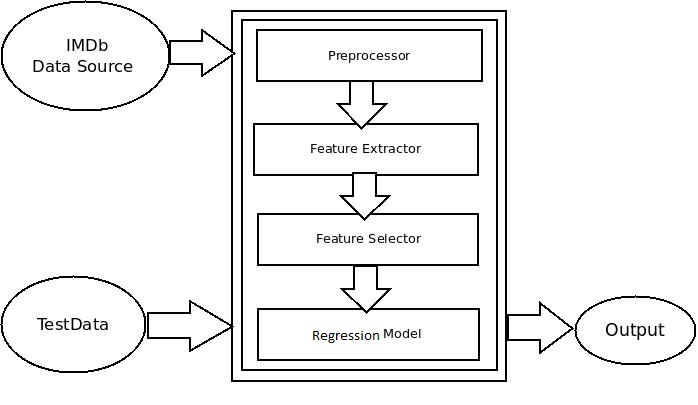
\includegraphics[scale=0.7]{Diagram.jpg}
  \caption{General Design}
\end{figure}
\section{Introduction}
The project can be mainly divided into two stages
\begin{description}
\item[$\bullet$ ]Dataset Collection and Preprocessing.
\item[$\bullet$ ]Construction of Regression Model.
\end{description}
\section{Dataset Collection and Preprocessing}
Dataset Collection is an important step in all machine learning problems. Preprocessing includes feature extraction and selection.
\subsection{Dataset Collection}
The initial dataset to be used will be collected from IMDb. It will consist of movies that were released from 2000 to 2012. Among these movies,we only selected the ones that were released in the United States and are in English, in the anticipation that we would be able to make more accurate predictions on these movies given that their reviews would also be in English.We removed movies which don't have any information about Box office details. 
\subsection{Preprocessing}


In preprocessing step we intent to eliminate training samples that have insufficient data. Also we intent to ensure that all the 19 genres in the IMDB database are well represented. We also want to filter the data in order to remove redundant and unnecessary information.
\subsection{Feature Selection}
\begin{figure}[htb!]
  \centering
      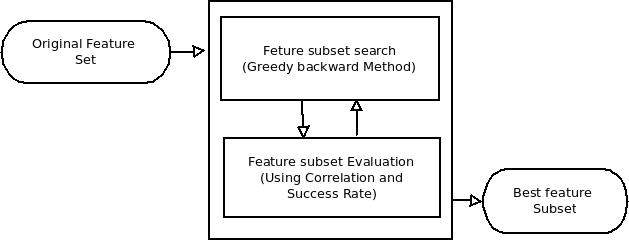
\includegraphics[scale=0.55]{featureselection.jpeg}
  \caption{Feature Selection}
\end{figure}
Here we look for correlation between all the different features under consideration and look for correlations with the target variable, ie movie revenue in dollars. We also look for correlation between the features themselves in order to avoid redundancy and irrelevant attributes. Also the extent of correlation is noted.Here we are using {\bf greedy 
backward procedure} to get best feature subset. The procedure starts with the
 full set of attributes.At each step, it removes the worst attribute remaining in the set.
At the end of the process, features that are not correlated to the target variable and those which are redundant are eliminated.

\section{Construction of Regression Model}
Supervised learning technique is adopted for this project.
We are using three models to predict the revenue and we will compare the performance of the different methods.




\subsection{Linear Regression Model}
In our first model, we use standard least-squares linear regression. To do this, we intend to use stochastic gradient descent. Once we have trained a set of feature weights, we could then generate gross revenue predictions as follows:
\centerline{ Gross = $\theta_{0}$ + $\theta_{1}$ * F$_1$ + $\theta_{2}$ * F$_2$ + ... + $\theta_{n}$ * F$_n$}\\	
where $\theta_i$ are the weights, F$_i$ are the features, and n is the number of features.\\
\subsection{Logistic Regression model}
We chose Logistic regression as our second method mainly because it generates a multi-class model with linear weights, most directly comparable to the feature weights given by linear regression. To define our classes we draw a histogram of movie revenues to create different buckets for prediction. These buckets are continuous ranges of movie revenues which covers the entire sample space.
\subsection{Support Vector Machine Regression Model}
SVMs can also be applied to regression problems.
SVM Regression try to find a function f(x)that has at most $\varepsilon$  deviation from the actually obtained targets y for all the training data, and at the same time is as flat as possibles. SVM Regression do not care about errors as long as they are less than $\varepsilon$ .We used linear kernel function to  map the data into a high dimensional feature space where linear regression is performed.
\clearpage
\chapter{WORK DONE}

\section{Obtaining The Data Set}
\begin{figure}[htb!]
  \centering
      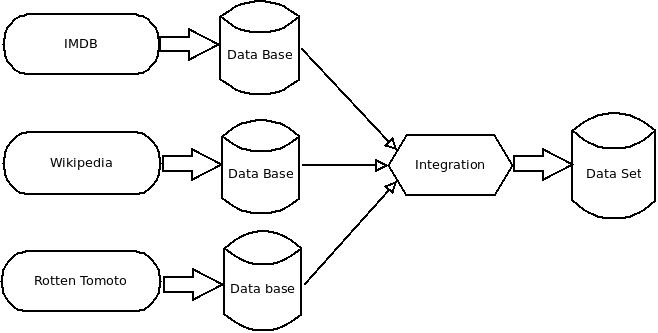
\includegraphics[scale=0.55]{data.jpeg}
  \caption{Data Collection and Integration}
\end{figure}
The data for a subset of movies,actors,reviews is provided by imdb via an alternative interface. Python scripts could be used to obtain data from IMDB. The data regarding each movie is spread over two web pages. The main page(imdb.com/title/movieid.html) and box office page.  
The data is also available at other websites like OMDB and Rotten Tomatoes in JSON format.
Eventually we faced a problem with Budget information.
Budget data is not provided by both IMDB and  Rotten Tomatoes. So we used wikipedia to obtain Budget details.
\section {Data Preprocessing}
The data we obtained are highly suseptible to noisy, missing and inconsistent data due to huge size and their likely origin from multiple, heterogeneous sources[9]. We mainly used IMDB and Rotten Tomatoes and Wikipedia. The main problem  with datasets were missing fields. To overcome this missing field problem we adopted a method which uses a measure of central tendency for the attribute. We used both mean and median as central tendency. Then removed duplicate entries.
\subsection {Data Integration}
Data obtained from three different resources IMDB, Wikipedia and Rotten Tomatoes was then  integrated into one database.
\subsection {Data Transformation}
In this step integrated data are transformed or consolidated so that the regression process may be more efficient and easier.
Dataset is mixed with both nominal and numeric attributes but for regression process we need all attributes to be numerical.
We used a measure of central tendency of Box office revenue to convert corresponding nominal attributes to numerical.
\subsection{Selecting feature Subset}
The dataset contained 20 features. We implemented a greedy backward procedure to reduce the dataset to the best feature subset. This resulted in a subset of 7 features.
\subsection{Measuring Sentiment Score From Reviews}
WE implemented a module to compute sentiment scores using a technique similar to the one used in the opinion finder project. The method involves assigning weights to commonly used adjectives to obtain an average weight.
\clearpage
\section{MACHINE LEARNING}
\subsection {Building a Linear Regression Model}
Using the method of Normal equation we built a linear regression model. We used data regarding 950 films  for training purpose and 100 for testing.Initially we had 17 features in the data set. After feature selection we chose a training set with the seven features that showed highest correlation to the target variable and low correlation among themselves. Correlation between features and cross validation on the training data were used as the performance matrix.


\subsection {Logistic Regression model}
   For logistic regression to apply we need to change the problem which is a regression problem to a classification problem. To achieve this we split the range of the target variable into a finite number of buckets of equal size. We found that the target variable takes values between \$2100 and \$436500000. We also found that only a few movies grossed over \$100 million. So we decided not to consider the movies that grossed over  \$100 million in the training set for the logistic regression model. We modelled the problem as a four class classification problem. The four classes were from \$0-\$25, \$25-\$50, \$50-\$75, \$75-\$100. There were a total of 876 movies in the data-set and we used 776 for training and 100 for testing. We used gradient descent algorithm to find the weights of the features.
\subsection {SVM with Linear Kernel}
Since Training data is not large as compared to number of features, we used linear kernel function. $\varepsilon$ was set to 0.1 and Hyperparameter C optimization was done using grid search.Grid search is exhaustive search through a manually specified subset of the hyperparameter space.Cross validation on the training was used as the performance matrix .The Optimum value for C was found to be 0.1 .
\\
\\

\section{WEB APPLICATION}
A web application was built using python to make results available to public.
\subsection {Google App engine}
Google App engine is used as the platform to run the code and is shared among the public to utilize the application.
\subsection {OMBD API}
Omdb API is used to collect the preliminary data set. Using this API we collected English movies from 2000 to 2010. We got around 25000 movies in the json format.
\subsection {Wikipedia}
Data set we collected using Omdb Api did not have the information regarding the budget of the films.To collect this information we used Wikipedia to collect budget data about films.
\clearpage


\chapter{RESULT}
The result we found out using Linear regression was about 51\% accurate. Where As for logistic regression we got 42.2\% accuracy which is a comparatively low result. SVM approach had a success rate of 39\%. The error tolerance for SVM and Linear regression was 20\%. For logistic regression the error tolerance was 12.5\%. Of all the 20 features in the data-set, budget, director, writer, actor1, actor2, gender, tomato reviews were found to be the most significant features.

\begin{center}
    \begin{tabular}{ | l | l | l | p{5cm} |}
    \hline
    Model & Linear Regression & Logistic Regression & SVM \\ \hline
    Tolerance & 20\% & 12.5\% & 20\% \\ \hline
    Success Rate & 50.7\% & 42.2\% & 39.0\% \\ \hline
    Correlation & 0.965 & - & 0.956 \\ \hline
    \end{tabular}
\end{center}



\chapter{CONCLUSION}
After building the three models we found out that the linear model represents the movie features most accurately. The success percentage for all models, while not good enough for industrial use, are in the close proximity of values obtained in previous studies. Some of the results obtained are better than that of some standard libraries and similar studies. Even though not good enough for industrial purposes the models built can be used in online applications.


A regression model which is supplied with a larger training set will be able to perform better. More data can be added to the training set over time as new information becomes available.

%% ADD data
\chapter{FUTURE WORKS}
\begin{description}
A larger training set is the key to improving the performance of the model. We need to consider additional features to achieve this. News analysis and plot analysis could be done and the information thus obtained could be added to the training set.

\end{description}

%\clearpage
\begin{thebibliography}{10}
\addcontentsline{toc}{chapter}{BIBLIOGRAPHY}
\bibitem{latexGuide} Richard O. Duda, Peter E. Hart, David G.
Stork,{\it Pattern Classification}, 2nd ed.NewYork: Wiley, 1973


\bibitem{latexMath}Sagar V. Mehta, Rose Marie Philip, Aju Thalappillil Scaria, "Predicting Movie Rating based on Text Reviews," Dept.Elect.Eng, Stanford Univ., California, December, 2011


\bibitem{latexGuide}Darin Im, Minh Thao, Dang Nguyen, "Predicting Movie Success in the U.S. market," Dept.Elect.Eng, Stanford Univ., California, December, 2011
 



\bibitem{latexMath}Suhaas Prasad, "Using Social Networks to improve Movie Ratings predictions,"
Dept.Elect.Eng, Stanford Univ., California, 2010

\bibitem{latexMath}Opinion Finder Project, University of Pittsburg,
Available: http://mpqa.cs.pitt.edu/opinionfinder/


\bibitem{latexMath}Andrew L. Maas, Raymond E. Daly, Peter T. Pham, Dan Huang,
Andrew Y. Ng, and Christopher Potts, "Learning Word Vectors for Sentiment Analysis,"In Proc. 49th Annual Meeting of the Association for Computational Linguistics, Oregon, 2011, pp 142$-$150


\bibitem{latexMath} Deniz Demir, Olga Kapralova, Hongze Lai, "Predicting IMDB Movie Ratings Using Google Trends," Dept.Elect.Eng, Stanford Univ., California, December, 2012

\bibitem{latexMath}W. Zhang and S. Skiena," Improving movie gross prediction through news analysis,", IEEE/WIC/ACM International Conference on Web Intelligence and Intelligent Agent Technology, Milan, 2009\\

\bibitem{latexMath} Jiawei Han, Micheline Kamber, Jian Pei,{\it  Data Mining Concepts and Techniques}, 3rd ed.MA:Elsevier, 2011, pp. 83-117
\end{thebibliography}
\end{document} to your LaTeX file where you want your
% title page.
%
%%%%%%%%%%%%%%%%%%%%%%%%%%%%%%%%%%%%%%%%%

%----------------------------------------------------------------------------------------
%	PACKAGES AND OTHER DOCUMENT CONFIGURATIONS
%----------------------------------------------------------------------------------------

\documentclass[12pt]{report}
\usepackage{graphicx}
\usepackage[section]{placeins}
\begin{document}

\begin{titlepage}

\newcommand{\HRule}{\rule{\linewidth}{0.5mm}} % Defines a new command for the horizontal lines, change thickness here

\center % Center everything on the page
 
%----------------------------------------------------------------------------------------
%	HEADING SECTIONS
%----------------------------------------------------------------------------------------
\textsc{\large Project Report On }\\[0.5cm] % Major heading such as course name % Minor heading such as course title

%----------------------------------------------------------------------------------------
%	TITLE SECTION
%----------------------------------------------------------------------------------------


{\Large  \bfseries EYE GAZE TRACKING
}\\[0.8cm] % Title of your document

\small \emph{Submitted in partial fulfillment of\\
        the requirements for the award of the degree of}
        \vspace{.2in}

       {\bf Bachelor of Technology \\in\\ Computer Science and Engineering}\\[0.2in]

 
%----------------------------------------------------------------------------------------
%	AUTHOR SECTION
%----------------------------------------------------------------------------------------
\textit{By}

\HRule \\[.2cm]
\begin{minipage}{0.4\textwidth}
\begin{flushleft} \large
Aravind Balakrishnan\\
Arun Abraham\\
Nikhil M S
\end{flushleft}
\end{minipage}
~
\begin{minipage}{0.4\textwidth}
\begin{flushright} \large
B100290CS\\
B100439CS\\
B100479CS\\
\end{flushright}
\end{minipage}\\[.5cm]

\HRule \\[0.2cm]

%----------------------------------------------------------------------------------------
%	Guidance
%----------------------------------------------------------------------------------------
\textit{\textit{Under the guidance of}}\\[0.1cm]
\textbf{\large Mrs. Lijiya A}\\[0.4cm]
%----------------------------------------------------------------------------------------
%	Image logo
%----------------------------------------------------------------------------------------

\includegraphics[scale=0.25]{nitc}\\
\Large { \textit \textbf Computer Science And Engineering}\\
 \large {NATIONAL INSTITUTE OF TECHNOLOGY CALICUT}
 Calicut, Kerala 673601
%----------------------------------------------------------------------------------------
%	DATE SECTION
%----------------------------------------------------------------------------------------

\textit{\large Winter Semester 2014}\\[3cm] % Date, change the \today to a set date if you want to be precise

%----------------------------------------------------------------------------------------
%	LOGO SECTION
%----------------------------------------------------------------------------------------

%\includegraphics{Logo}\\[1cm] % Include a department/university logo - this will require the graphicx package
 
%----------------------------------------------------------------------------------------

\vfill % Fill the rest of the page with whitespace

\end{titlepage}
%------------------------------------Certificate---------------------------------------------------

\newpage
\thispagestyle{empty}

\begin{center}

\huge{Computer Science and Engineering}\\
\normalsize
\textsc{National Institute of Technology Calicut}\\[2cm]

\emph{\LARGE Certificate}\\[2.0cm]
\end{center}
\normalsize This is to certify that the project work entitled "Eye Gaze Tracking", submitted by the following students to National Institute of Technology Calicut towards partial fulfilment of the requirements of the award of Degree Of Bachelor of Technology in Computer Science and Engineering is a bonafide record of the work carried out by them under my supervision and guidance.\\[.5cm]

\begin{table}[h]
\centering
\begin{tabular}{lr}
Roll No & Names of Students  \\ \hline
\\
B100290CS & Aravind Balakrishnan \\
B100439CS & Arun Abraham \\ 
B100479CS & Nikhil M S \\
\\
\hline
\end{tabular}
\end{table}

\vfill


% Bottom of the page
\begin{flushright}
Mrs. Lijiya A\\
(Project Guide)\\[1.5cm]
Gopakumar G\\
(Course Coordinator)\\
\end{flushright}

\begin{flushleft}
Place: Calicut \\
Date:

\end{flushleft}

%------------------------------------End of Certificate----------------------------------------------

\v
\begin{abstract}

 American film studios collectively produce several hundred movies every year, making the United States the third most prolific producer of films in the world. The budget of these movies is of the order of hundreds of millions of dollars, making their box office success absolutely essential for the survival of the industry. Knowing which movies are likely to succeed and which are likely to fail before the release could benefit the production houses greatly as it will enable them to focus their advertising campaigns which itself cost millions of dollars, accordingly. And it could also help them to know when it is most appropriate to release a movie by looking at the overall market. So the prediction of movie success is of great importance to the industry.

Machine learning algorithms are widely used to make predictions such as growth in the stock market, demand for products, nature of tumors etc. The goal of this project is to use data available in the Internet to predict the revenue of the movies and the critical success as well. Critical success will be represented by the IMDB ratings. The main challenge is to find the appropriate features to be considered for making the predictions. This problem is modelled as a linear regression problem.

\end{abstract}
\clearpage
\chapter*{PROBLEM STATEMENT}
The aim of the project is to predict the box office revenue and critical success of new Hollywood movies using machine learning techniques. The IMDB rating after at least one month after the release is considered as the index of critical success. We intend to make two predictions, one before the release and the second after one week of release. 
\clearpage
\pagenumbering{roman}
\tableofcontents
\newpage
\pagenumbering{arabic}
\chapter{INTRODUCTION}
In the United States of America 1000s of films are released every year.Since the 1920s, the American film industry has grossed more money every year than that of any other country. Cinema in America is a multi-billion dollar industry where even individual films earn over a billion dollars. Large production houses control most of the film industry, with billions of dollars spent on advertisements alone. Advertising campaigns contribute heavily to the total budget of the movies. Sometimes the investment results in heavy losses to the producers.
Warner Brothers, one of the largest production houses had a fall in their revenues last year despite the inflation and the increased number of movies released. If it was somehow possible to know beforehand the likelihood of success of the movies, the production houses could adjust the release of their movies so as to gain maximum profit. They could use the predictions to know when the market is dull and when its not.
 This shows a dire need for such a software to be developed. Many have tried to accomplish this goal of predicting movie revenues. Techniques such as social media sentiment analysis have been used in the past. None of the studies thus far has succeeded in suggesting a model good enough to be used in the industry.
In this project we attempt to use IMDB data to predict the gross revenue of the movies as well as their IMDB rating.


\clearpage
\chapter{LITERATURE SURVEY}
Lot of work has been done in the area and too many people have attempted to use statistics in combination with machine learning algorithms to predict various entities.\\
\begin{itemize}
\item Opinion Finder, a project conducted at University of Pittsburg [5] attempted to  use tweets to predict market sentiments. Their approach was to give different weightage to the adjectives in the tweets. They assigned values ranging from +2 to -2 to certain words and took the average weight to make predictions.
\item In their paper presented in the 49th annual meeting for ACN in 2011 [6]. Andrew Ng, Christopher Potts and their colleagues pointed out the importance of using a mix of supervised and unsupervised  approaches to learn word vectors capturing semantic term–document information as well as rich sentiment content.
\item Independant works conducted by Matts Forsell and Darin Im [3] attempted to predict Movie Revenues and had different success rates. Forsell’s prediction used a slightly more extensive training set than Im’s. But the prediction success was lower. Darin Im used a smaller training set, however used data that was from very recent movies. Forsell noted that error rates were significantly higher in predicting success of movies with budget lower than 100 million. 
\item Project conducted by Deniz Demir and Olga Kapralova at Stanford [7] used google trends statistics to improve movie gross prediction. They tried two different approaches. In one they used google trends statistics in combination with google adwords, in the other they used google trends statistics only.Their data set consisted of 800 movies only. This was mainly because google trends statistics  is available from 2004 onwards only. They used Logistic Regression, SVM and Multilayer perceptron approaches. All three approaches yielded average success rate close to 50 percentage. However, SVM method correctly predicted 98\% of the low rated movies but its success rate for high rated movies(ratings above 6) was a meagre 11\%.

\item Wenbin Zhang at Sony Brook University,NY used news analysis [8] alone to predict movie revenues without considering any other parameters including IMDB data. In their approach they tried to find correlations between various parameters and movie revenues. They found that prediction models using news data only can achieve similar performance to models using IMDB data, especially for high-grossing movies. They concluded that adding news analysis features can improve performance of predictions that use IMDB data alone.
\end{itemize}
\clearpage

\chapter{DESIGN}
\begin{figure}[h!]
  \centering
      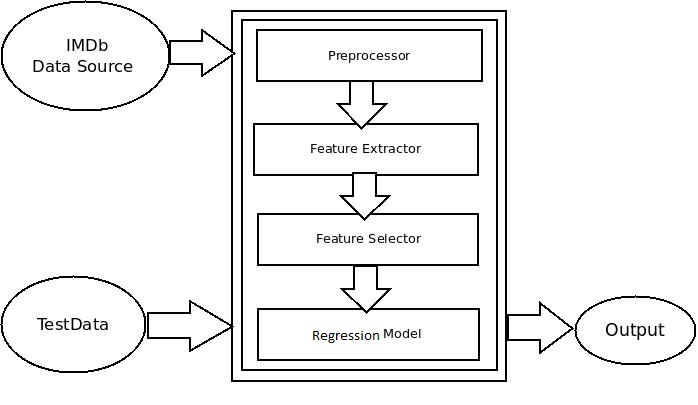
\includegraphics[scale=0.7]{Diagram.jpg}
  \caption{General Design}
\end{figure}
\section{Introduction}
The project can be mainly divided into two stages
\begin{description}
\item[$\bullet$ ]Dataset Collection and Preprocessing.
\item[$\bullet$ ]Construction of Regression Model.
\end{description}
\section{Dataset Collection and Preprocessing}
Dataset Collection is an important step in all machine learning problems. Preprocessing includes feature extraction and selection.
\subsection{Dataset Collection}
The initial dataset to be used will be collected from IMDb. It will consist of movies that were released from 2000 to 2012. Among these movies,we only selected the ones that were released in the United States and are in English, in the anticipation that we would be able to make more accurate predictions on these movies given that their reviews would also be in English.We removed movies which don't have any information about Box office details. 
\subsection{Preprocessing}


In preprocessing step we intent to eliminate training samples that have insufficient data. Also we intent to ensure that all the 19 genres in the IMDB database are well represented. We also want to filter the data in order to remove redundant and unnecessary information.
\subsection{Feature Selection}
\begin{figure}[htb!]
  \centering
      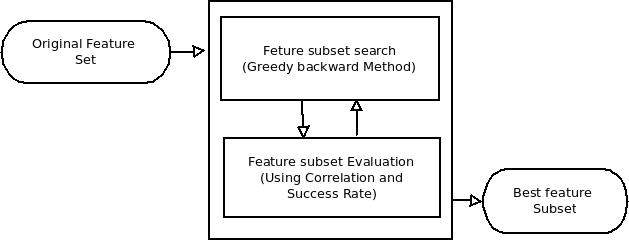
\includegraphics[scale=0.55]{featureselection.jpeg}
  \caption{Feature Selection}
\end{figure}
Here we look for correlation between all the different features under consideration and look for correlations with the target variable, ie movie revenue in dollars. We also look for correlation between the features themselves in order to avoid redundancy and irrelevant attributes. Also the extent of correlation is noted.Here we are using {\bf greedy 
backward procedure} to get best feature subset. The procedure starts with the
 full set of attributes.At each step, it removes the worst attribute remaining in the set.
At the end of the process, features that are not correlated to the target variable and those which are redundant are eliminated.

\section{Construction of Regression Model}
Supervised learning technique is adopted for this project.
We are using three models to predict the revenue and we will compare the performance of the different methods.




\subsection{Linear Regression Model}
In our first model, we use standard least-squares linear regression. To do this, we intend to use stochastic gradient descent. Once we have trained a set of feature weights, we could then generate gross revenue predictions as follows:
\centerline{ Gross = $\theta_{0}$ + $\theta_{1}$ * F$_1$ + $\theta_{2}$ * F$_2$ + ... + $\theta_{n}$ * F$_n$}\\	
where $\theta_i$ are the weights, F$_i$ are the features, and n is the number of features.\\
\subsection{Logistic Regression model}
We chose Logistic regression as our second method mainly because it generates a multi-class model with linear weights, most directly comparable to the feature weights given by linear regression. To define our classes we draw a histogram of movie revenues to create different buckets for prediction. These buckets are continuous ranges of movie revenues which covers the entire sample space.
\subsection{Support Vector Machine Regression Model}
SVMs can also be applied to regression problems.
SVM Regression try to find a function f(x)that has at most $\varepsilon$  deviation from the actually obtained targets y for all the training data, and at the same time is as flat as possibles. SVM Regression do not care about errors as long as they are less than $\varepsilon$ .We used linear kernel function to  map the data into a high dimensional feature space where linear regression is performed.
\clearpage
\chapter{WORK DONE}

\section{Obtaining The Data Set}
\begin{figure}[htb!]
  \centering
      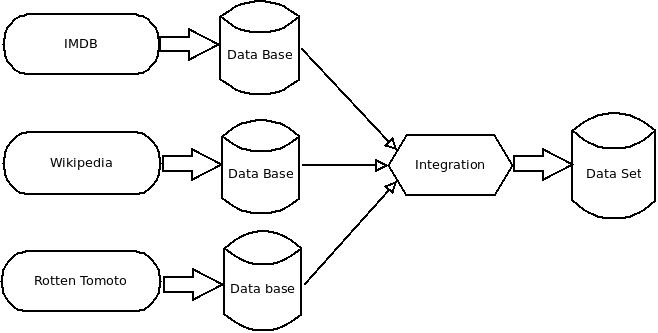
\includegraphics[scale=0.55]{data.jpeg}
  \caption{Data Collection and Integration}
\end{figure}
The data for a subset of movies,actors,reviews is provided by imdb via an alternative interface. Python scripts could be used to obtain data from IMDB. The data regarding each movie is spread over two web pages. The main page(imdb.com/title/movieid.html) and box office page.  
The data is also available at other websites like OMDB and Rotten Tomatoes in JSON format.
Eventually we faced a problem with Budget information.
Budget data is not provided by both IMDB and  Rotten Tomatoes. So we used wikipedia to obtain Budget details.
\section {Data Preprocessing}
The data we obtained are highly suseptible to noisy, missing and inconsistent data due to huge size and their likely origin from multiple, heterogeneous sources[9]. We mainly used IMDB and Rotten Tomatoes and Wikipedia. The main problem  with datasets were missing fields. To overcome this missing field problem we adopted a method which uses a measure of central tendency for the attribute. We used both mean and median as central tendency. Then removed duplicate entries.
\subsection {Data Integration}
Data obtained from three different resources IMDB, Wikipedia and Rotten Tomatoes was then  integrated into one database.
\subsection {Data Transformation}
In this step integrated data are transformed or consolidated so that the regression process may be more efficient and easier.
Dataset is mixed with both nominal and numeric attributes but for regression process we need all attributes to be numerical.
We used a measure of central tendency of Box office revenue to convert corresponding nominal attributes to numerical.
\subsection{Selecting feature Subset}
The dataset contained 20 features. We implemented a greedy backward procedure to reduce the dataset to the best feature subset. This resulted in a subset of 7 features.
\subsection{Measuring Sentiment Score From Reviews}
WE implemented a module to compute sentiment scores using a technique similar to the one used in the opinion finder project. The method involves assigning weights to commonly used adjectives to obtain an average weight.
\clearpage
\section{MACHINE LEARNING}
\subsection {Building a Linear Regression Model}
Using the method of Normal equation we built a linear regression model. We used data regarding 950 films  for training purpose and 100 for testing.Initially we had 17 features in the data set. After feature selection we chose a training set with the seven features that showed highest correlation to the target variable and low correlation among themselves. Correlation between features and cross validation on the training data were used as the performance matrix.


\subsection {Logistic Regression model}
   For logistic regression to apply we need to change the problem which is a regression problem to a classification problem. To achieve this we split the range of the target variable into a finite number of buckets of equal size. We found that the target variable takes values between \$2100 and \$436500000. We also found that only a few movies grossed over \$100 million. So we decided not to consider the movies that grossed over  \$100 million in the training set for the logistic regression model. We modelled the problem as a four class classification problem. The four classes were from \$0-\$25, \$25-\$50, \$50-\$75, \$75-\$100. There were a total of 876 movies in the data-set and we used 776 for training and 100 for testing. We used gradient descent algorithm to find the weights of the features.
\subsection {SVM with Linear Kernel}
Since Training data is not large as compared to number of features, we used linear kernel function. $\varepsilon$ was set to 0.1 and Hyperparameter C optimization was done using grid search.Grid search is exhaustive search through a manually specified subset of the hyperparameter space.Cross validation on the training was used as the performance matrix .The Optimum value for C was found to be 0.1 .
\\
\\

\section{WEB APPLICATION}
A web application was built using python to make results available to public.
\subsection {Google App engine}
Google App engine is used as the platform to run the code and is shared among the public to utilize the application.
\subsection {OMBD API}
Omdb API is used to collect the preliminary data set. Using this API we collected English movies from 2000 to 2010. We got around 25000 movies in the json format.
\subsection {Wikipedia}
Data set we collected using Omdb Api did not have the information regarding the budget of the films.To collect this information we used Wikipedia to collect budget data about films.
\clearpage


\chapter{RESULT}
The result we found out using Linear regression was about 51\% accurate. Where As for logistic regression we got 42.2\% accuracy which is a comparatively low result. SVM approach had a success rate of 39\%. The error tolerance for SVM and Linear regression was 20\%. For logistic regression the error tolerance was 12.5\%. Of all the 20 features in the data-set, budget, director, writer, actor1, actor2, gender, tomato reviews were found to be the most significant features.

\begin{center}
    \begin{tabular}{ | l | l | l | p{5cm} |}
    \hline
    Model & Linear Regression & Logistic Regression & SVM \\ \hline
    Tolerance & 20\% & 12.5\% & 20\% \\ \hline
    Success Rate & 50.7\% & 42.2\% & 39.0\% \\ \hline
    Correlation & 0.965 & - & 0.956 \\ \hline
    \end{tabular}
\end{center}



\chapter{CONCLUSION}
After building the three models we found out that the linear model represents the movie features most accurately. The success percentage for all models, while not good enough for industrial use, are in the close proximity of values obtained in previous studies. Some of the results obtained are better than that of some standard libraries and similar studies. Even though not good enough for industrial purposes the models built can be used in online applications.


A regression model which is supplied with a larger training set will be able to perform better. More data can be added to the training set over time as new information becomes available.

%% ADD data
\chapter{FUTURE WORKS}
\begin{description}
A larger training set is the key to improving the performance of the model. We need to consider additional features to achieve this. News analysis and plot analysis could be done and the information thus obtained could be added to the training set.

\end{description}

%\clearpage
\begin{thebibliography}{10}
\addcontentsline{toc}{chapter}{BIBLIOGRAPHY}
\bibitem{latexGuide} Richard O. Duda, Peter E. Hart, David G.
Stork,{\it Pattern Classification}, 2nd ed.NewYork: Wiley, 1973


\bibitem{latexMath}Sagar V. Mehta, Rose Marie Philip, Aju Thalappillil Scaria, "Predicting Movie Rating based on Text Reviews," Dept.Elect.Eng, Stanford Univ., California, December, 2011


\bibitem{latexGuide}Darin Im, Minh Thao, Dang Nguyen, "Predicting Movie Success in the U.S. market," Dept.Elect.Eng, Stanford Univ., California, December, 2011
 



\bibitem{latexMath}Suhaas Prasad, "Using Social Networks to improve Movie Ratings predictions,"
Dept.Elect.Eng, Stanford Univ., California, 2010

\bibitem{latexMath}Opinion Finder Project, University of Pittsburg,
Available: http://mpqa.cs.pitt.edu/opinionfinder/


\bibitem{latexMath}Andrew L. Maas, Raymond E. Daly, Peter T. Pham, Dan Huang,
Andrew Y. Ng, and Christopher Potts, "Learning Word Vectors for Sentiment Analysis,"In Proc. 49th Annual Meeting of the Association for Computational Linguistics, Oregon, 2011, pp 142$-$150


\bibitem{latexMath} Deniz Demir, Olga Kapralova, Hongze Lai, "Predicting IMDB Movie Ratings Using Google Trends," Dept.Elect.Eng, Stanford Univ., California, December, 2012

\bibitem{latexMath}W. Zhang and S. Skiena," Improving movie gross prediction through news analysis,", IEEE/WIC/ACM International Conference on Web Intelligence and Intelligent Agent Technology, Milan, 2009\\

\bibitem{latexMath} Jiawei Han, Micheline Kamber, Jian Pei,{\it  Data Mining Concepts and Techniques}, 3rd ed.MA:Elsevier, 2011, pp. 83-117
\end{thebibliography}
\end{document}